\documentclass[tikz,border=10pt]{standalone}
\usepackage{tikz}
\usetikzlibrary{positioning}
\usepackage{tikz-feynman}
\begin{document}
	
	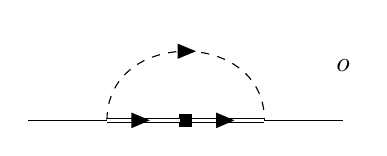
\begin{tikzpicture}[
		decuplet/.style={ % 自定义一个重子的双线
			double distance=1pt,
			postaction={decorate}, decoration={
				markings, mark=at position .6 with {
					\arrow{Triangle[angle=40:2pt 3]}
				},
			}
		}
		]
		\begin{feynman}
	     
	     
			%% fig o
			\vertex(o1) at (0,0);
			\vertex[right =1cm  of o1] (o2);
			\vertex[right =2cm  of o1,square dot,anchor=center] (o3){};
			\vertex[right =3cm  of o1] (o4);
			\vertex[right =4cm  of o1] (o5);
			\node[above =0.5 of o5] {$o$};
		
		
			
			% 对各个顶点连线
			\diagram*{
				{
					[edge=plain]
                    (o1)-- (o2) -- (o3)--(o4)--(o5),		
			},
				% 介子连线
				{
					[edge= charged scalar]
					(o2) --[half left](o4),
			}
			};
			%% 添加重子双线
			\draw[decuplet]  (o2) -- (o3);
			\draw[decuplet]  (o3) -- (o4);
				\end{feynman}
	\end{tikzpicture}
	
\end{document}
